\clearpage
\section{镜头外的灯牌照亮白墙}

把一盏灯牌架在白墙前面，让发光的一侧朝墙。相机也朝墙，但画面只取灯牌左侧的一小块。把场景里的点光源全部关掉，这块白墙原本会变成黑色。要让它亮起来，从墙面出发的光线就得找到镜头外的灯牌，并带回打中那个位置的颜色。

沿墙面法线朝向的半球取一条射线，找到它打中的第一块三角形。如果这块表面会发光，就按交点的 UV 找到纹素，先从 sRGB 转为线性 RGB，再乘材质中的发光颜色与强度。单面灯牌只有正面发光；双面灯牌的背面也可以照亮墙。\href{https://registry.khronos.org/glTF/specs/2.0/glTF-2.0.html#material-emissivetexture}{glTF 2.0，发光贴图}

\begin{center}
\begin{tabular}{@{}cccc@{}}

\includegraphics[width=.20\linewidth]{../../../output/profiling/emissive-gi/reference.png}&
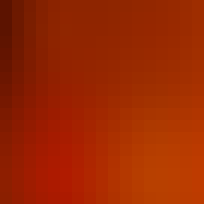
\includegraphics[width=.20\linewidth]{../../../output/profiling/emissive-gi/live-three.png}&

\includegraphics[width=.20\linewidth]{../../../output/profiling/emissive-gi/live-sixteen.png}&

\includegraphics[width=.20\linewidth]{../../../output/profiling/emissive-gi/baked.png}\\
面积积分 & 每方向 3 条 & 每方向 16 条 & 烘焙后
\end{tabular}
\end{center}
{\small 左图按灯牌的位置与两个纹素独立算出。后三图是 Vulkan 输出的同一小块墙，原始大小均为 $17\times17$。中间两图取第 24 帧。四张图都用 $1-e^{-2L}$ 调亮并转成 sRGB，下面的数值直接读原始线性颜色。\par}

这块测试灯牌宽 1.2、高 1，与墙平行，两者相隔一个场景单位。把灯牌分成 $128\times96$ 个小方块。站在墙上一点 $x$ 看某个小块 $y$，离得远，它占的视角就小；斜着看，它看起来也会窄。设两点距离是 $r$，连线与两侧法线的夹角分别是 $\theta_x,\theta_y$，小块面积为 $\Delta A$。让每个小块发出的颜色 $L_e(y)$ 乘上这些比例，再乘白墙的漫反射率 $\rho=0.8$，把各块的贡献加起来，就有了参考值。
\[
  L_o(x)\;\approx\;\frac{\rho}{\pi}\sum_y L_e(y)
    \frac{\cos\theta_x\cos\theta_y}{r^2}\,\Delta A .
\]
灯牌的左纹素是纯红色 255，右纹素的绿色是 128。绿色解码后约为 0.216，乘绿色因子 0.5 和强度 4，约为 0.432。这两个数指灯牌自身发出的颜色。传到墙面还要经过上式，整块墙的参考平均值降到了 $(0.215215,0.014061,0)$。GPU 从每个墙面像素发出 2,048 条射线，得到 $(0.215356,0.014110,0)$。ReSTIR GI 每像素每帧只有一个新候选，512 帧平均是 $(0.213964,0.014929,0)$。\href{https://pbr-book.org/4ed/Light_Sources/Area_Lights}{PBRT 第四版 §12.4}

DDGI 会先让附近的探针观察灯牌，再用这些探针估计墙上的光。每个方向从 3 条射线增到 16 条后，上图的深浅变化平缓了一些。把相邻像素的红色差与面积积分作比较，误差从 0.01024 降到 0.00475；但整幅画的红色平均值也从 0.21282 变为 0.17053。增加射线能减轻起伏，探针之间插值造成的偏差仍在。烘焙后这块墙的平均红色为 0.19981。关掉应用再打开，289 个像素的四个浮点分量与之前完全相同。要继续改善大墙上的色斑，可以先让窄灯牌占据的方向更容易被取到，再用同一机位检查相邻像素和平均颜色两个指标。

\href{run:../../tests/EmissiveGICheck.h}{面积积分与 Vulkan 回归}\quad\href{run:../profiling/emissive-gi/measurements.csv}{逐项读数}
